%% rnaastex.cls is the classfile used for Research Notes. It is derived
%% from aastex61.cls with a few tweaks to allow for the unique format required.
\documentclass{rnaastex}
\usepackage{amsmath, amssymb, bm}
\DeclareMathOperator*{\argmin}{arg\,min}

\newcommand{\todo}[3]{{\color{#2} \emph{#1} TO DO: #3}}
\newcommand{\zetodo}[1]{\todo{ZE}{cyan}{#1}}
\newcommand{\rpm}{\sbox0{$1$}\sbox2{$\scriptstyle\pm$}
\raise\dimexpr(\ht0-\ht2)/2\relax\box2 }

%% Define new commands here
\newcommand\latex{La\TeX}

\newcommand{\chicago}{Department of Astronomy and Astrophysics, University of
Chicago, 5640 S. Ellis Ave, Chicago, IL 60637, USA}
\newcommand{\sagan}{Sagan Fellow}

\begin{document}

\title{Point Spread Function Photometry: The Poisson Likelihood and Unbiased Estimations}


%% Note that the corresponding author command and emails has to come
%% before everything else. Also place all the emails in the \email
%% command instead of using multiple \email calls.
\correspondingauthor{Jos\'e Vin\'icius de Miranda Cardoso}
\email{j.demirandacardoso@nasa.gov}

\author{Jos\'e Vin\'icius de Miranda Cardoso}
\affiliation{NASA Ames Research Center, Moffett Blvd, Mountain View, CA 94035, USA}
\affiliation{Bay Area Environmental Research Institute, 625 2nd St Ste. 209, Petaluma, CA 94952}

\author{Geert Barentsen}
\affiliation{NASA Ames Research Center, Moffett Blvd, Mountain View, CA 94035, USA}
\affiliation{Bay Area Environmental Research Institute, 625 2nd St Ste. 209, Petaluma, CA 94952}

\author{Benjamin T. Montet}
\altaffiliation{\sagan}
\affiliation{\chicago}

\author{Michael Gully-Santiago}
\affiliation{NASA Ames Research Center, Moffett Blvd, Mountain View, CA 94035, USA}
\affiliation{Bay Area Environmental Research Institute, 625 2nd St Ste. 209, Petaluma, CA 94952}
%% Note that RNAAS manuscripts DO NOT have abstracts.
%% See the online documentation for the full list of available subject
%% keywords and the rules for their use.
\keywords{point spread function --- statistical estimation --- photometry}

%% Start the main body of the article. If no sections in the
%% research note leave the \section call blank to make the title.
\section*{}

Photometry from charged-couple devices (CCDs) lies at the core of astronomical
observations.  When targets are isolated, aperture photometry
can be performed by summing the flux across an appropriate selection of pixels.
In crowded regions, conversely, targets are not disjoint and more complicated
techniques such as point spread function (PSF) fitting or difference imaging
photometry need to be employed~\citep[e.g. see][]{heasley:1999}.

PSF photometry consists of fitting the parameters of a PSF model to the images
of stars.  Traditionally, maximum likelihood esimates of the parameters
are obtained by minimizing the  $\chi^2$ statistic, inspired by the
implications of the Central Limit Theorem~\citep{grimmett:2001}.

In this note, we advocate that the $\chi^2$ statistic might not be adequate
for PSF photometry for two main reasons: (I) the assumption of Gaussian
distributed data is only compatible with the nature of pixel data in an
assymptotic sense; (II) the $\chi^2$ statistic yields a maximum likelihood
estimator (MLE) for the total number of counts which is biased, and therefore
it is only compatible with aperture photometry in an assymptotic sense.

Here, we report that under Poissonian data distributed assumptions,
and for a very general family of PSF models, the total number of counts
obtained using PSF photometry, employing the maximum likelihood estimator, is
equivalent to aperture photometry. As it will be shown, this equivalency is not
valid if Gaussian distributed data is assumed.

We begin by stating the underlying statistical assumptions.
Given an image as a collection of $n$ independent \emph{non-identically}
distributed random variables $\bm{Y} \triangleq \{Y_i\}_{i=1}^{n}$ (pixels),
such that $\mathbb{E}\left[Y_i\right] = \lambda_i(\bm{\Theta})$, in which
$\lambda_i$ is the PSF model evaluated at the $i$-th pixel, and $\bm{\Theta}$
is a $\Lambda$-valued random vector, where $\Lambda \subseteq \mathbb{R}^p$ is
a compact set that encodes the information about, say, the total number of
counts and center positions of the PSF model.

Assuming further that, for a given vector of stellar parameters
$\bm{\Theta} = \bm{\theta}$, $Y_i$ follows a Poisson distribution, then the
joint conditional likelihood function of a stellar image $\bm{Y}$ can be
expressed as~\citep{grimmett:2001}
\begin{align}
    P(\bm{Y} = \bm{y} | \bm{\Theta} = \bm{\theta}) =
    \prod_{i=1}^{n} p(y_i | \bm{\theta}) =
    \prod_{i=1}^{n}\dfrac{\lambda_i^{y_i}(\bm{\theta})}{y_i!}\exp{-\lambda_i(\bm{\theta})} =
    \exp\left({-\sum_{i=1}^{n}\lambda_i(\bm{\theta})}\right)\prod_{i=1}^{n}\dfrac{\lambda_i^{y_i}(\bm{\theta})}{y_i!}.
\end{align}

Perhaps of more practical interest is the log likelihood function
\begin{equation}
    \log P(\bm{Y} = \bm{y} | \bm{\Theta} = \bm{\theta}) =
    \sum_{i=1}^{n}\left(- \lambda_i(\bm{\theta})
    + y_i\log\lambda_i(\bm{\theta}) - \log y_i !\right).
\end{equation}

Then, the MLE can be formulated as
\begin{align}
    \bm{\theta}^{*}(\bm{y}) = \argmin_{\bm{\theta} \in \Lambda}
    \sum_{i=1}^{n}\left(\lambda_i(\bm{\theta}) - y_i\log\lambda_i(\bm{\theta})\right),
\end{align}
which must satisfy the following system of differential equations
\begin{equation}
    \sum_{i=1}^{n}\dfrac{\partial \lambda_i(\bm{\theta})}{\partial \theta_j}
    \left(1 - \dfrac{y_i}{\lambda_i(\bm{\theta})} \right)
    \Bigr|_{\substack{\bm{\theta}=\bm{\theta}^{*}(\bm{y})}} = 0,
    ~\mathrm{for}~j=1, 2, ..., p,
    \label{eq:partial_eqs}
\end{equation}
assuming that $\bm{\theta}^{*}(\bm{y})$ is an interior point of $\Lambda$.

Now, assume that the vector of stellar parameters $\bm{\theta}$ takes the
following form $\bm{\theta} \triangleq (\alpha, \bm{x})$, where $\alpha$
is the total number of counts and $\bm{x} \triangleq (x_1, x_2)$ is the
coordinate of the center of the PSF. Further, assume that the PSF model can be
factorized as follows
\begin{equation}
    \lambda_i(\bm{\theta}) = \alpha\cdot\psi_i(\bm{x}),
    \label{eq:psf_model}
\end{equation}
where $\psi_i(\bm{x})$ is the normalized PSF model centered at $\bm{x}$ at the
\textit{i}-th pixel, such that $\sum_{i=1}^{n}\psi_i(\bm{x})=1$.

Therefore,
\begin{equation}
    \dfrac{\partial{\lambda_i(\bm{\theta})}}{\partial \alpha} = \psi_i(\bm{x})~\text{and}~
    \dfrac{\partial^2{\lambda_i(\bm{\theta})}}{\partial \alpha^2} = 0.
    \label{eq:partial_flux}
\end{equation}

Substituting (\ref{eq:psf_model}) and (\ref{eq:partial_flux}) into
(\ref{eq:partial_eqs}), it follows that
\begin{align}
    \sum_{i=1}^{n} \psi_i(\bm{x}^{*})\left(1 - \dfrac{y_i}{\alpha^{*}
    \cdot\psi_i(\bm{x}^{*})} \right) &= \sum_{i=1}^{n} \left(\psi_i(\bm{x}^{*})
    -  \dfrac{y_i}{\alpha^{*}}\right) = 0~~~\Leftrightarrow~~~\alpha^{*} = \sum_{i=1}^{n} y_i.
    \label{eq:tada}
\end{align}

Furthermore, computing the derivative of the left hand side
of~(\ref{eq:partial_eqs}), \textit{i.e.}, the second-order derivative of the
negative of the log likelihood function, with respect to $\alpha$, and
evaluating it at $\alpha^{*}$, it follows that
\begin{align}
    \sum_{i=1}^{n}\left\{\dfrac{\partial^2 \lambda_i\left(\bm{\theta}\right)}{\partial \alpha^2}
    - \dfrac{y_i}{\lambda_i\left(\bm{\theta}\right)}\left[\dfrac{\partial^2 \lambda_i
    \left(\bm{\theta}\right)}{\partial \alpha^2} - \dfrac{1}{\lambda_i\left(\bm{\theta}\right)}
    \left(\dfrac{\partial \lambda_i\left(\bm{\theta}\right)}{\partial \alpha}\right)^2\right]\right\}
    \Bigr|_{\substack{\alpha=\alpha^{*}}} = \sum_{i=1}^{n}\dfrac{y_i}{\alpha^2}
    \Bigr|_{\substack{\alpha=\alpha^{*}}} = \dfrac{1}{\alpha^{*}} > 0
    \label{eq:partial2_eqs}
\end{align}
which proves our proposition. Note that this result does not require any
specific structural form of $\lambda_i$ other than it increases linearly with
the total number of counts $\alpha$ for a given fixed position $\bm{x}$.

Furthermore, the MLE for the total number of counts has the following nice
properties: (\textrm{I}) it is an unbiased estimator and (\textrm{II}) its
variance attains the minimum possible bound (Cram\'er-Rao Lower
Bound~\citep{bobrovsky:1987}) in the Fisher information sense. The first
property may be verified by taking the expectation value of (\ref{eq:tada}),
which follows that
\begin{equation}
    \mathbb{E}\left[\alpha^{*}\right] = \sum_{i=1}^{n}\mathbb{E}[Y_i] =
    \sum_{i=1}^{n} \lambda_i(\bm{\theta}) =
    \sum_{i=1}^{n} \alpha\cdot\psi_i(\bm{x}) = \alpha.
\end{equation}
To verify the second property, note that $\alpha^{*}$ is the sum of independent
Poisson random variables, therefore, $var\left[\alpha^{*}\right] =
\mathbb{E}\left[\alpha^{*}\right] = \alpha$.

Note that, under the widely adopted assumption that the data is Gaussian
distributed (corresponding to a $\chi^2$ likelihood function),
the solution for $\alpha^{*}$ would be
\begin{equation}
    \alpha^{*} = \dfrac{\sum_{i=1}^{n}y_i \psi_i(\bm{x}^{*})}{\sum_{i=1}^{n}\psi^2_i(\bm{x}^{*})},
\end{equation}
for which, properties (I) and (II) are not known to hold.

It is worth noticing that, whenever the number of counts is high (which often
is the case around the center of the PSF), the Poisson density does converge to
a Gaussian density, and therefore those two approaches are equivalent.

However, for pixels at the tail of the PSF or low signal-to-noise targets,
where the number of counts is small, the Gaussian approximation might
yield residuals that are nonnegligeble for practical scenarios such as transit
photometry.

As a practical exercise, we apply PSF photometry on the target
\texttt{KIC10053146} of NASA's Kepler Mission. \texttt{KIC10053146} is a
20th magnitude isolated star which has an average flux of $260 e^{-}s^{-1}$ in
the brightest pixel.

Using the assumption that the data is Poisson distributed, we obtain a mean
residual value at the two brightest pixels across 4000 cadences of
$9.35~\rpm~4.45~e^{-}s^{-1}$. The same analysis with Gaussian likelihood
assumption yields $10.11~\rpm~5.76~e^{-}s^{-1}$. The mean residuals
considering all 30 pixels was $-2.25\cdot 10^{-5}~\rpm~12.58~e^{-}s^{-1}~$,
and $0.99~\rpm~12.59~e^{-}s^{-1}~$ for the Poisson and Gaussian assumptions,
respectively.

\begin{figure}[!htb]
    \centering
    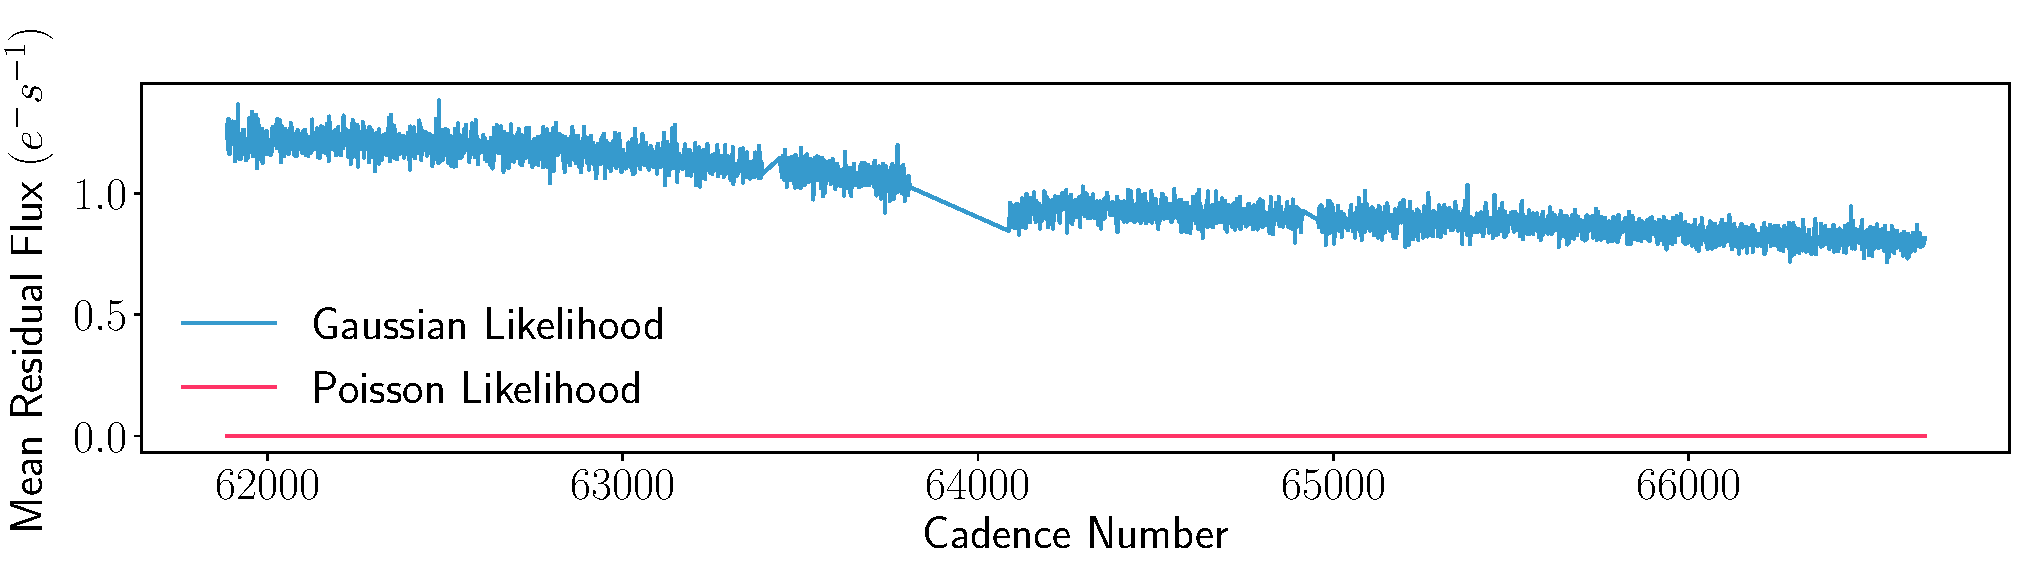
\includegraphics[scale=.5]{comparison.pdf}
    \caption{Mean residuals per cadence of PSF photometry using Poisson
             Likelihood (red) and Gaussian Likelihood (blue).}
\end{figure}

\acknowledgments This work acknowledges the use of the following computational
tools: \texttt{numpy}~\citep{numpy}, \texttt{scipy}~\citep{scipy},
\texttt{astropy}~\citep{astropy}, \texttt{pyke}~\citep{pyke},
and \texttt{jupyter}~\citep{jupyter}.
A \texttt{jupyter} notebook intented to reproduce the example aforementioned is
available at: \url{https://www.github.com/mirca/geerts-conjecture}.
Work by B.T.M. was performed under contract with the Jet Propulsion Laboratory (JPL) funded by 
NASA through the Sagan Fellowship Program executed by the NASA Exoplanet Science Institute.

\begin{thebibliography}{}
    \bibitem[Heasley(1999)]{heasley:1999} Heasley, J.~N., Point-Spread Function
        Fitting Photometry, 1999, Astronomical Society of the Pacific Conference Series.
    \bibitem[Grimmet et al.(2001)]{grimmett:2001} Grimmett, R.~G.,
        Stirzaker D.~R., Probability and Random Processes, 2001, Oxford University Press.
    \bibitem[Bobrovsky et al. (1987)]{bobrovsky:1987} Bobrovsky, B.~Z.,
        Mayer-Wolf E., Zakai M., Some Classes of Global Cram\'er-Rao Bounds, 1987,
        The Annals of Statistics, Vol. 15, No. 4, 1421 -- 1438.
    \bibitem[Jones et al. (2001)]{scipy} Jones, E., Oliphant T.,
        Peterson P., et al., \texttt{SciPy}: Open source scientific tools
        for \texttt{Python}.
    \bibitem[van der Walt et al. (2011)]{numpy} van der Walt S., Colbert S.~C.,
        Varoquaux G., The NumPy Array: a structure for efficient numerical
        computation, 2011, Computing in Science \& Engineering, 13, 22--30.
    \bibitem[Hunter (2007)]{matplotlib} Hunter, J. D., Matplotlib: A 2D graphic
        environment, 2007, Computing in Science \& Engineering, 9, 90--95.
    \bibitem[AstroPy Project (2017)]{astropy} AstroPy Project, Submitted to ApJ, 2017.
    \bibitem[PyKE Contributors (2017)]{pyke} PyKE Contributors, PyKE: Kepler,
        $\mathcal{K}\mathit{2}$ \& TESS Data Analysis Tools, 2017,
        \url{http://doi.org/10.5281/zenodo.835584}.
    \bibitem[Perez et al. (2007)]{jupyter} P\'erez F., Granger B.~E.,
        \texttt{IPython}: a system for interactive scientific computing, 2007,
        Computing in Science and Engineering, 9, 21--29.
\end{thebibliography}

\end{document}

